%# -*- coding: utf-8 -*-
% !TeX encoding = UTF-8 Unicode
% !TeX spellcheck = en_US
% !TeX TS-program = xelatex
%~ \XeTeXinputencoding "UTF-8"
% vim:ts=4:sw=4
%
% 以上设定默认使用 XeLaTex 编译,并指定 Unicode 编码,供 TeXShop 自动识别

\chapter{Introduction}

There're three types of environment be supported by the software,
which are single host bash, hadoop, and myhadoop.

In hadoop environment, the system will need HDFS to store both the data and executable for all of nodes involved.
\begin{itemize}
  \item executable: such as ns2 C++ binary and its support files
  \item data: config files and TCL scripts for the specific simulation
\end{itemize}
Once a node start to run the simulation, the map-reduce script should load the binary files from HDFS to local host first,
then read a global config file for environment settings,
and read a config file for that simulation to continue simulation.

While in myhadoop case, the data and executable are not necessary to be stored in HDFS since there's share file system for the HPC.
But the user should also be warned because some type of network file system (NFS) will downgrade the simulation speed if the simulator write the data to the NFS directly.
One of the trade-off is to copy the config files from the NFS to a directory of local disks and run the simulator on that directory and copy the data back to the NFS after finishing the simulation.

To overcome all of these challenges mentioned above,
we integrate the following functions in the software:
\begin{itemize}
  \item An abstract interface for the file system: it supports copy files, move files, print files on the standard output, find files etc. So that the software can support local files and HDFS files in a restricted computing environment (we're not system administrator and can't install various file system driver by ourselves.).
  \item use local disks to store data temporally: to speed up the simulation.
\end{itemize}



Figure \ref{fig:mrnativestack} shows the structure of the framework.
The script \texttt{plboot-pbs.sh} is to set up the environment variables for hadoop run in PBS,
and the script \texttt{plboot-lan.sh} is for the hosts in LAN.
these two scripts will generate \texttt{myhadoop.conf} to be used by myhadoop,
optimized parameters in \texttt{mapred-site.xml}, and/or \texttt{yarn-site.xml} for hadoop,

\begin{figure}\centering
  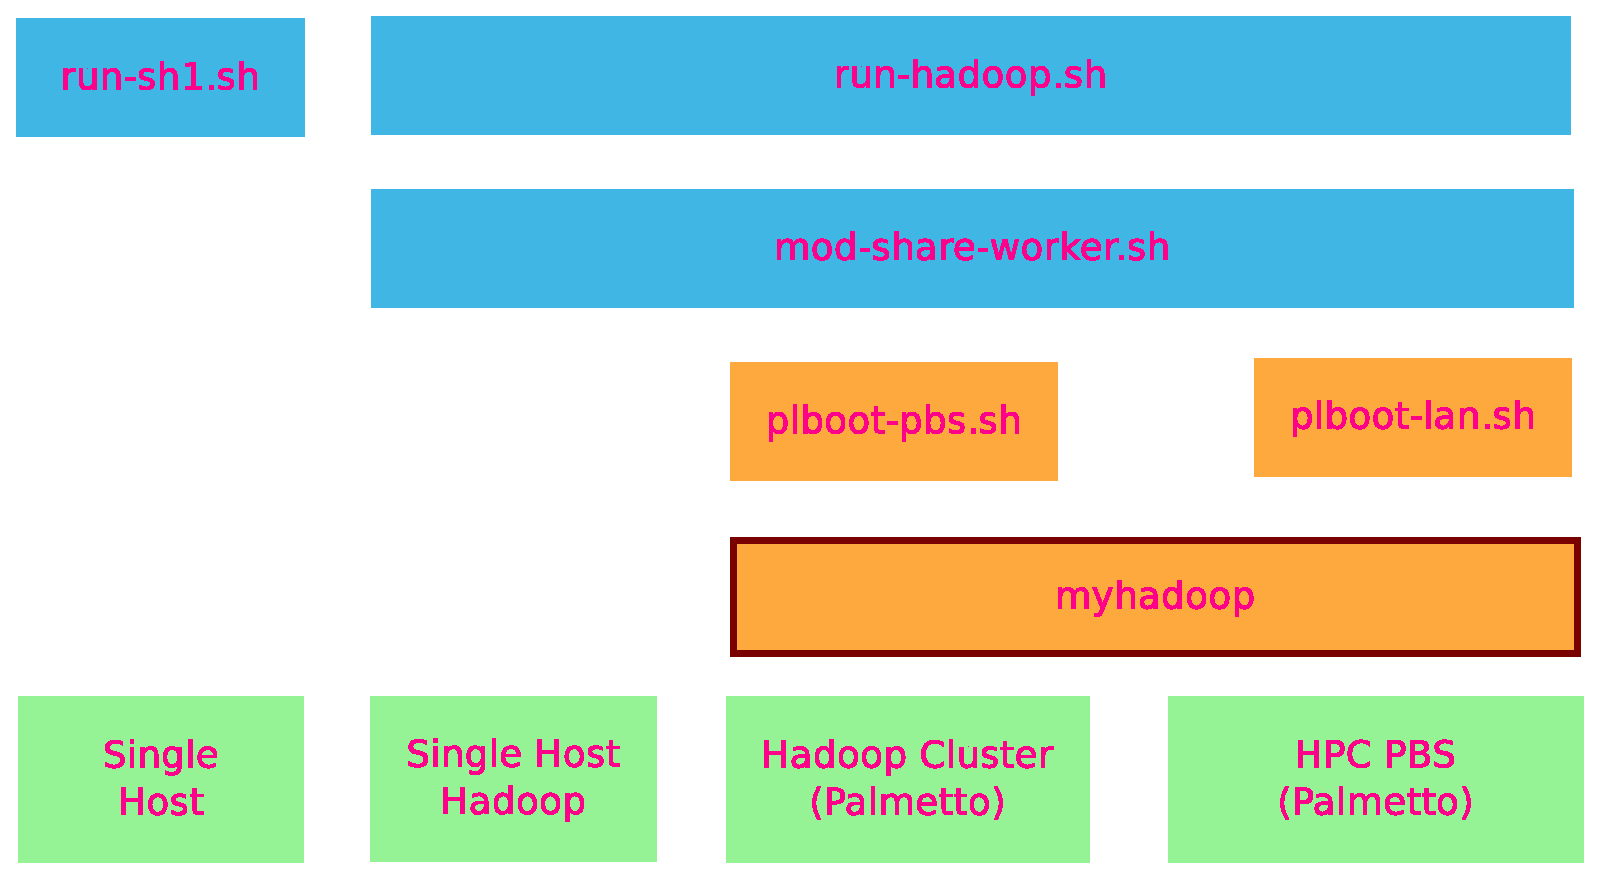
\includegraphics[width=0.7\textwidth]{mrnative-stack}
  \caption{The stack of the mrnative}\label{fig:mrnativestack}
\end{figure}



